\section{Chapter 6}
\subsection{Set A}

\begin{enumerate}
    \item $f$ is bijective: $f^{-1}(x) = (x - 4)/3$.\\ Range: $\mathbb{R}$.

    \item $f$ is bijective: $f^{-1}(x) = \sqrt[3]{x - 1}$.\\ Range: $\mathbb{R}$.

    \item $f$ is not injective: $|x| = |-x| = x$ for any $x \in \mathbb{R}$. $f$ is surjective: $|y| = y$, for any $y \in \mathbb{R}$.\\ Range: $\{x \in \mathbb{R}: x \geqslant 0\}$.

    \item $f$ is not injective: $f(-1) = f(2) = 2$. $f$ is surjective because it is continuous and unbounded.\\ Range: $\mathbb{R}$.

    \item $f$ is bijective: 
        
       \[
        f^{-1}(x) = 
            \begin{cases}
                x & \text{if $x$ is rational} \\
                \frac{x}{2} & \text{if $x$ is irrational}
            \end{cases}
        \]

      Range: $\mathbb{R}$.

    \item $f$ is injective, but not surjective: for any odd number $y$, there is no $x$ such that $f(x) = y$.\\ Range: $\{x \in \mathbb{Z}: x = 2k, \text{for all $k \in \mathbb{Z}$}\} \cup \{x \notin \mathbb{Z}\}$.
\end{enumerate}


\subsection{Set B}
\begin{enumerate}
    \item $f$ is bijective: $f^{-1}(x) = \ln(x)$.

    \item $f$ is bijective: $f^{-1}(x) = \arctan(x)$.

    \item $f$ is not injective: given $f(x_1) = f(x_2)$, $x_1$ and $x_2$ can independently be any number in $\{y: \in \mathbb{R}: x_i - 1 < y \leqslant x_i\}$. $f$ is surjective: any integer maps to itself.

    \item $f$ is bijective: $f^{-1} = f$.

    \item $f(n) = 2n$.
\end{enumerate}

\subsection{Set C}
\begin{enumerate}
    \item $f$ is not injective: take $f(x, y_1) = f(x, y_2)$ even when $y_1 \ne y_2$. $f$ is surjective: any element $x \in A$ is the image of $(x, y)$, for any $y \in B$.

    \item $f$ is bijective: $f^{-1} = f$.

    \item $f$ is injective, but not surjective: none of the elements in the set $\{x \in B: x \ne b\}$ is an image of any element in $A$.

    \item $f$ is bijective: $f^{-1}(x) = a^{-1}x$.

    \item $f$ is bijective: $f^{-1} = f$.

    \item $f$ is not bijective: take, for example the group of Table \ref{tab:op-exercise-5G1}; in that case, $a^2 = b^2 = e$. $f$ is not surjective: take, for example $\angled{\mathbb{Z}, +}$; in this case $f(x) = 2x$, which means that odd numbers are not the image of any element in $\mathbb{Z}$.
\end{enumerate}

\subsection{Set D}
\begin{enumerate}
    \item $(f \circ g)(x) = \sin(e^x)$; $(g \circ f)(x) = e^{\sin(x)}$.\\
    $f \circ g: \mathbb{R} \to \mathbb{R}$; $g \circ f: \mathbb{R} \to \mathbb{R}$.

    \item $(g \circ f)(x, y) = y$.\\
    $g \circ f: A \times B \to B$.

    \item $(g \circ f)(x) = \ln(1/x)$; $f \circ g$ would be defined as $(f \circ g)(x) = 1/\ln x$, but $(f \circ g)(1) = 1/0$, which is undefined.\\
    $g \circ f: (0, 1) \to \mathbb{R}$.

    \item $f \circ g = g \circ f$, which consists of spelling every word backwards and interchanging the letters a with o, i with u and e with y.\\
    $g \circ f: \text{Latin alphabet} \to \text{Latin alphabet}$.

    \item $f \circ g = \begin{bmatrix}
        a & b & c & d \\
        c & a & c & a \\
    \end{bmatrix}$, 
    $g \circ f = \begin{bmatrix}
        a & b & c & d \\
        b & b & b & b \\
    \end{bmatrix}$.\\
    $g \circ f: \{a, b, c, d\} \to \{a, b, c, d\}$.

    \item $(f \circ g)(x) = abx$; $(f \circ g)(x) = bax$;\\
    $f \circ g: G \to G$; $g \circ f: G \to G$.
\end{enumerate}

\subsection{Set E}
\begin{enumerate}
    \item $f^{-1} = f$.

    \item $f^{-1}(x) = \ln x$.

    \item $f^{-1}(x) = \sqrt[3]{x - 1}$.

    \item $f^{-1}(x) = \begin{cases}
        x/2 & \text{if $x$ is rational} \\
        x/3 & \text{if $x$ is irrational}
    \end{cases}$

    \item $f^{-1} = \begin{bmatrix}
        3 & 1 & 2 & 4 \\
        a & b & c & d
    \end{bmatrix}$

    \item $f^{-1}(x) = a^{-1}x$
\end{enumerate}

\subsection{Set F}
\begin{enumerate}
    \item The whole committee.

    \item If $f$ is injective, then every element of $A$ must map to a different element of $A$. In other words, every element in $A$ is image of some other element in $A$. Therefore $f$ is surjective.

    \item Let us assume that $f$ is not injective, which corresponds to saying that at least one element is the image of at least two different elements in the domain. In that case, the number of elements in the range would be smaller than the number of elements in $A$, contradicting the fact that $f$ is surjective. Therefore, $f$ is injective.

    \item $f: \mathbb{Z} \to \mathbb{Z}$, defined by $f(x) = 2x$, is injective but not surjective.\\
    $f: \mathbb{R} \to \mathbb{Z}$, defined by $f(x) = $ the least integer greater than or equal to $x$, is surjective but not injective.

    \item $n^n$ functions, out of which $n!$ functions are bijective.
\end{enumerate}

\subsection{Set G}
\begin{enumerate}
    \item Let us assume that $f$ is not injective. That means that there are at least two distinct elements $x_1, x_2 \in A$ such that $f(x_1) = f(x_2)$. In that case, $g(f(x_1)) = g(f(x_2))$, contradicting the fact that $g \circ f$ is injective. Therefore, $f$ is injective.

    \item Let us assume that $g$ is not surjective. That means that there is at least one element in $C$ that is not an image of any element in $B$ under $g$. Then that element cannot possibly be an image of any element in $A$ under $g \circ f$, contradicting the fact that $g \circ f$ is surjective. Therefore, $g$ is surjective.

    \item Take $f, g: \mathbb{Z} \to \mathbb{Z}$, defined by $f(x) = 2x$ and $g(x) = -x$; then $(g \circ f)(x) = -2x$, which is not bijective, since odd numbers are not images under this function.

    \item For every $x$, $f(x)$ is defined and so is $g(f(x)) = x$. Therefore $g = f^{-1}$ and $f$ is bijective.
\end{enumerate}

\subsection{Set H}
In the following items, $*$ means ``any symbol'', and $!x$ means ``any symbol except $x$''. $0$ is always the initial state and, in the diagrams, the green circle represents the acceptance state. All others are failure states.
\begin{enumerate}
    \item $A = \{a, b, c, d\}$; $S = \{0, 1, 2, 3, 4\}$; machine table: see Table \ref{tab:machine-3as}; diagram: see Figure \ref{fig:threeas}.
    \begin{table}[!ht]
        \centering
        \begin{tabular}{l|ll}
        Present state & a & !a \\ \hline
        0             & 1 & 0  \\
        1             & 2 & 1  \\
        2             & 3 & 2  \\
        3             & 4 & 3  \\
        4             & 4 & 4 
        \end{tabular}
        \caption{State machine for input consisting of exactly 3 a's}
        \label{tab:machine-3as}
    \end{table}
    \begin{figure}[!ht]
        \centering
        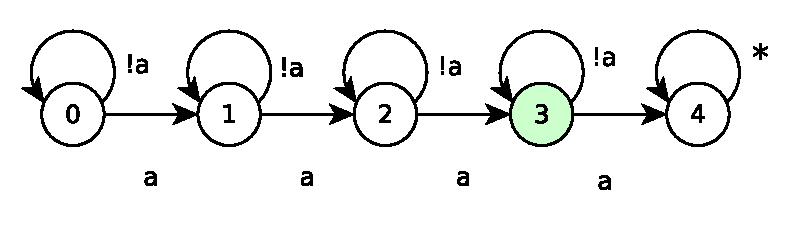
\includegraphics[scale=0.5]{diagrams/threeas.pdf}
        \caption{State machine for input consisting of exactly 3 a's}
        \label{fig:threeas}
    \end{figure}
    
    \item $A = \{a, b, c, d\}$; $S = \{0, 1, 2, 3\}$; machine table: see Table \ref{tab:machine-at-least-3as}; diagram: see Figure \ref{fig:atleast3as}
    \begin{table}[!ht]
        \centering
        \begin{tabular}{l|ll}
        Present state & a & !a \\ \hline
        0             & 1 & 0  \\
        1             & 2 & 1  \\
        2             & 3 & 2  \\
        3             & 4 & 3  \\
        4             & 4 & 4 
        \end{tabular}
        \caption{State machine for input consisting of at least 3 a's}
        \label{tab:machine-at-least-3as}
    \end{table}
    \begin{figure}[!ht]
        \centering
        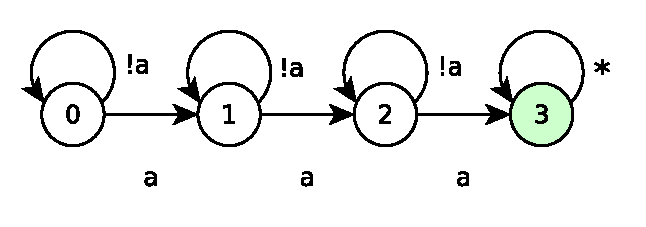
\includegraphics[scale=0.5]{diagrams/atleast3as.pdf}
        \caption{State machine for input consisting of at least 3 a's}
        \label{fig:atleast3as}
    \end{figure}

    \item $A = \{0, 1, 2, 3, 4\}$; $S = \{0, 1, 2, 3, 4\}$; machine table: see Table \ref{tab:add-modulo-5}; diagram: see Figure \ref{fig:add-modulo-5}
    \begin{table}[]
        \centering
        \begin{tabular}{l|lllll}
        Present state & 0 & 1 & 2 & 3 & 4 \\ \hline
        0             & 0 & 1 & 2 & 3 & 4 \\
        1             & 1 & 2 & 3 & 4 & 0 \\
        2             & 2 & 3 & 4 & 0 & 1 \\
        3             & 3 & 4 & 0 & 1 & 2 \\
        4             & 4 & 0 & 1 & 2 & 3
        \end{tabular}
        \caption{State machine for addition modulo 5}
        \label{tab:add-modulo-5}
    \end{table}
    \begin{figure}[!ht]
        \centering
        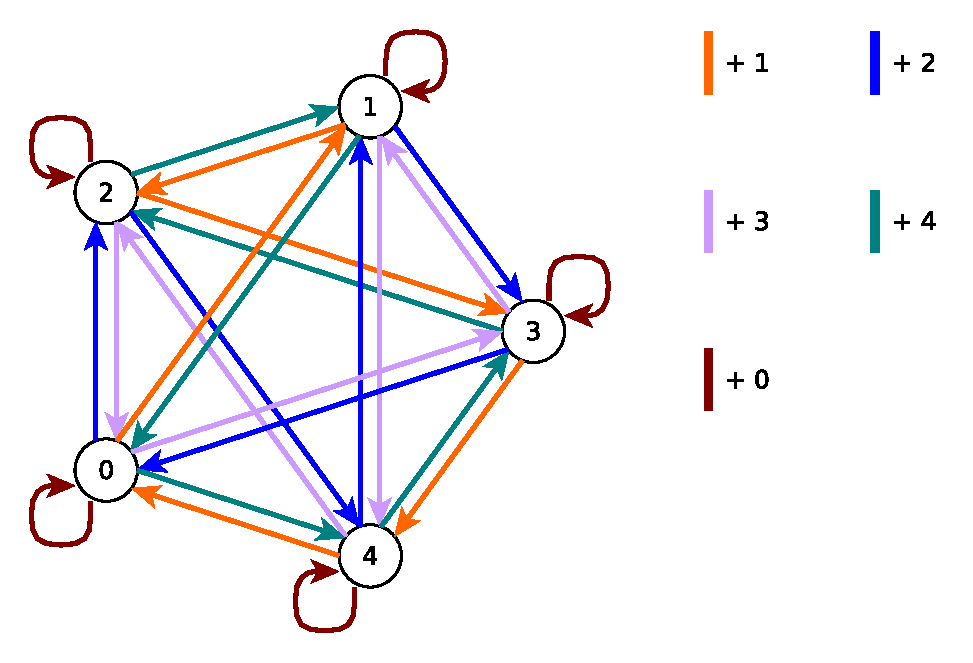
\includegraphics[scale=0.5]{diagrams/add-modulo-5.pdf}
        \caption{State machine for addition modulo 5}
        \label{fig:add-modulo-5}
    \end{figure}

    \item $A = \{0, 1\}$; $S = \{0, 1, 2, 3\}$; machine table: see Table \ref{tab:ends-in-111}; diagram: see Figure \ref{fig:ends-in-111}.
    \begin{table}[]
        \centering
        \begin{tabular}{l|ll}
        Present state & 0 & 1 \\ \hline
        0             & 0 & 1 \\
        1             & 0 & 2 \\
        2             & 0 & 3 \\
        3             & 0 & 0
        \end{tabular}
        \caption{State machine for binary string ending in 111}
        \label{tab:ends-in-111}
    \end{table}
    \begin{figure}[!ht]
        \centering
        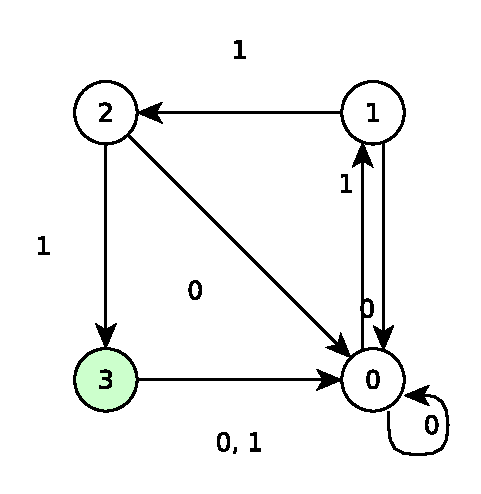
\includegraphics[scale=0.5]{diagrams/ends-in-111.pdf}
        \caption{State machine for binary string ending in 111}
        \label{fig:ends-in-111}
    \end{figure}

    \item \begin{enumerate}[label=(\alph*)]
        \item 
        $\bar{\alpha}(s_0, 000) = s_0$\quad
        $\bar{\alpha}(s_0, 100) = s_1$\\
        $\bar{\alpha}(s_0, 001) = s_1$\quad
        $\bar{\alpha}(s_0, 101) = s_0$\\
        $\bar{\alpha}(s_0, 010) = s_1$\quad
        $\bar{\alpha}(s_0, 110) = s_0$\\
        $\bar{\alpha}(s_0, 011) = s_0$\quad
        $\bar{\alpha}(s_0, 111) = s_1$

        \item 
        $\bar{\alpha}(s_0, 00) = s_0$\quad
        $\bar{\alpha}(s_1, 00) = s_1$\\
        $\bar{\alpha}(s_0, 01) = s_1$\quad
        $\bar{\alpha}(s_1, 01) = s_0$\\
        $\bar{\alpha}(s_0, 10) = s_1$\quad
        $\bar{\alpha}(s_1, 10) = s_0$\\
        $\bar{\alpha}(s_0, 11) = s_0$\quad
        $\bar{\alpha}(s_1, 11) = s_1$
    \end{enumerate}

    \item
        \begin{enumerate}[label=(\alph*)]
            \item 
            $\mathbf{x} = 01001$:\quad $T_\mathbf{x}(s_0) = s_0$\quad $T_\mathbf{x}(s_1) = s_1$\\
            $\mathbf{x} = 10011$:\quad $T_\mathbf{x}(s_0) = s_1$\quad $T_\mathbf{x}(s_1) = s_0$\\
            $\mathbf{x} = 01010$:\quad $T_\mathbf{x}(s_0) = s_0$\quad $T_\mathbf{x}(s_1) = s_1$

            \item In the case of $M_1$, $T_\mathbf{x}$ either maps the initial state to the same state if the weight of $\mathbf{x}$ is even and to the opposite state otherwise. So, there are only two functions.

            \item In general, let $n$ be the number of $a$'s in a given $\mathbf{x}$; then $T_\mathbf{x}(s_i) = s_j$, in which $j = \max(i + n, 4)$.

            \item We can think of $T_\mathbf{x}(s_i)$ as a fuction $f(\mathbf{x}, i) = \sum\limits_{b \in \mathbf{x}} (b \mod 4) + (i \mod 4)$. Since $\mathbf{x}$ determines the function and there are only 5 possible values for the term that includes it in $f$, there are therefore only 5 distinct transition functions in this case.
        \end{enumerate}
\end{enumerate}

\subsection{Set I}
\begin{enumerate}
    \item see Table \ref{tab:automaton-mz4} and Figure \ref{fig:automaton-mz4}.
    
    \begin{table}[]
        \centering
        \begin{tabular}{l|llll}
        Present state & 0 & 1 & 2 & 3 \\ \hline
        0             & 0 & 1 & 2 & 3 \\
        1             & 1 & 2 & 3 & 0 \\
        2             & 2 & 3 & 0 & 1 \\
        3             & 3 & 0 & 1 & 2
        \end{tabular}
        \caption{Automaton $M(\mathbb{Z}_4)$}
        \label{tab:automaton-mz4}
    \end{table}
    \begin{figure}
        \centering
        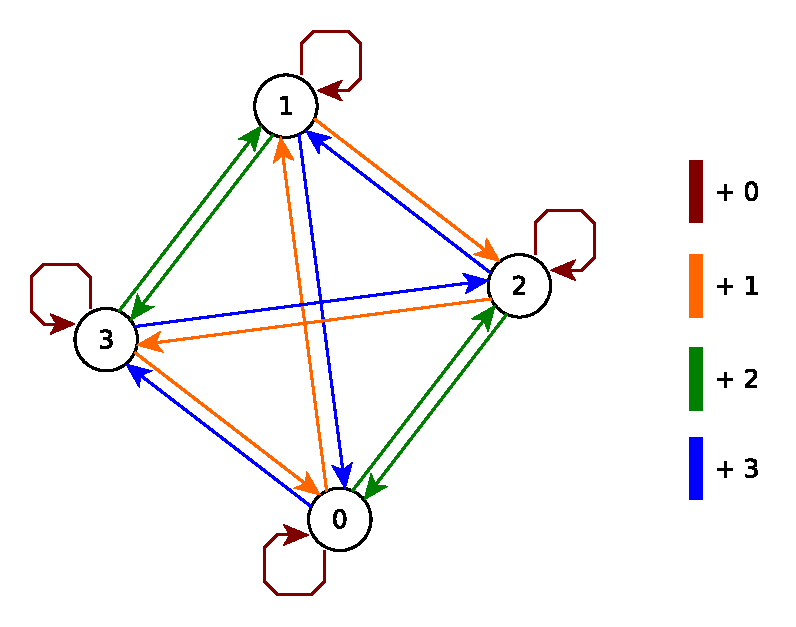
\includegraphics[scale=0.5]{diagrams/automaton-mz4.pdf}
        \caption{Automaton $M(\mathbb{Z}_4)$}
        \label{fig:automaton-mz4}        
    \end{figure}

    \item \begin{minipage}{0.5\textwidth}
        \centering
        $e = \begin{bmatrix}
            1 & 2 & 3 \\
            1 & 2 & 3 \\
        \end{bmatrix}$\\
        $a = \begin{bmatrix}
            1 & 2 & 3 \\
            1 & 3 & 2 \\
        \end{bmatrix}$\\
        $b = \begin{bmatrix}
            1 & 2 & 3 \\
            3 & 1 & 2 \\
        \end{bmatrix}$\\
        $c = \begin{bmatrix}
            1 & 2 & 3 \\
            3 & 2 & 1 \\
        \end{bmatrix}$\\
        $d = \begin{bmatrix}
            1 & 2 & 3 \\
            2 & 3 & 1 \\
        \end{bmatrix}$\\
        $f = \begin{bmatrix}
            1 & 2 & 3 \\
            2 & 1 & 3 \\
        \end{bmatrix}$\\
    \end{minipage}
    \begin{minipage}{0.5\textwidth}
        \centering
        \begin{tabular}{l|llllll}
            $\circ$ & $e$ & $a$ & $b$ & $c$ & $d$ & $f$ \\ \hline
            $e$       & $e$ & $a$ & $b$ & $c$ & $d$ & $f$ \\
            $a$       & $a$ & $e$ & $f$ & $d$ & $c$ & $b$ \\
            $b$       & $b$ & $c$ & $d$ & $f$ & $e$ & $a$ \\
            $c$       & $c$ & $b$ & $a$ & $e$ & $f$ & $d$ \\
            $d$       & $d$ & $f$ & $e$ & $a$ & $b$ & $c$ \\
            $f$       & $f$ & $d$ & $c$ & $b$ & $a$ & $e$
        \end{tabular}
    \end{minipage}\\        
    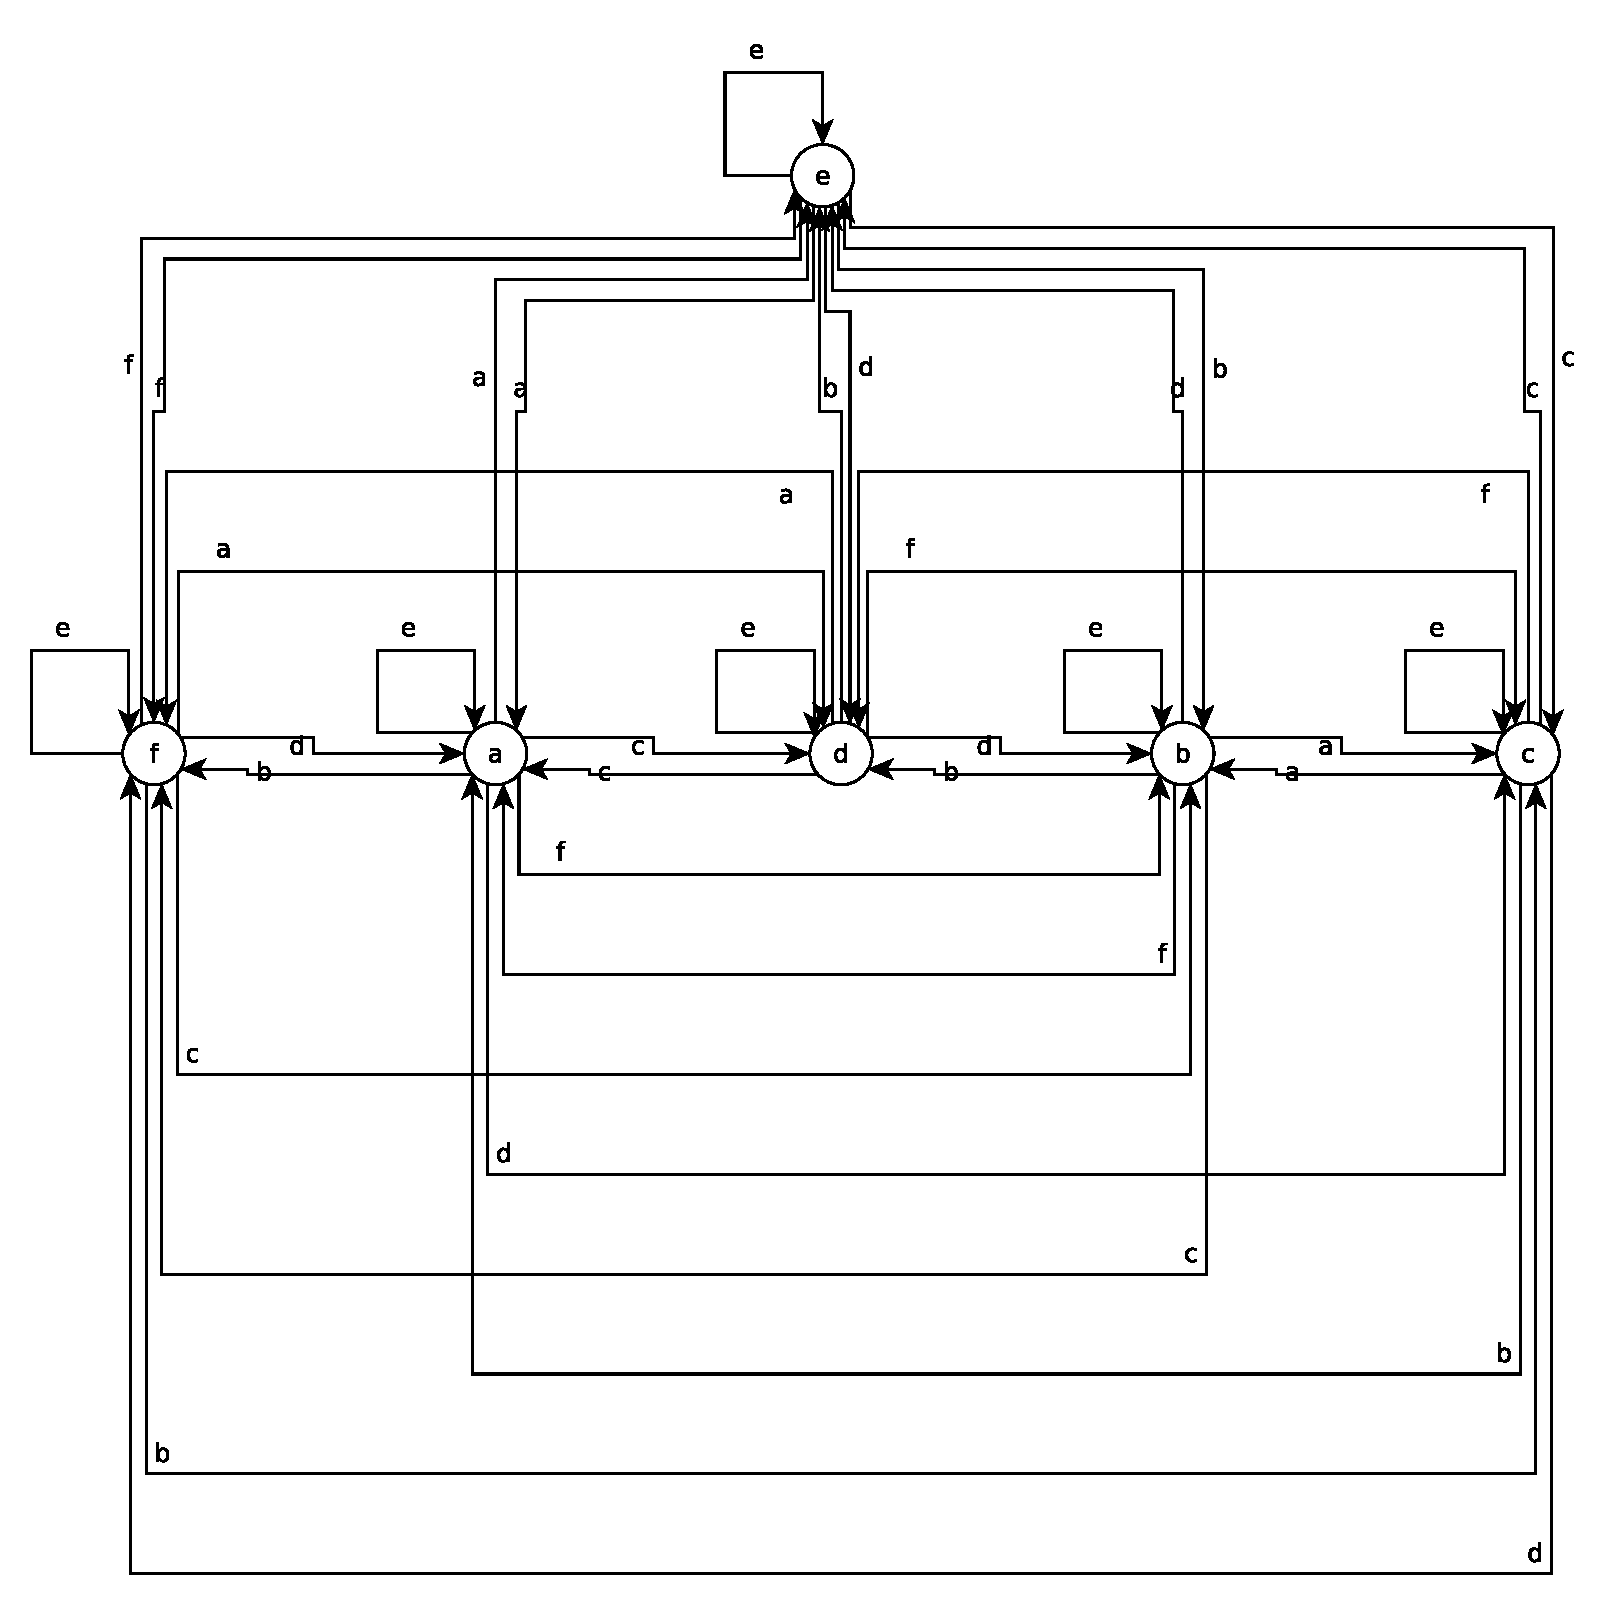
\includegraphics[scale=0.5]{diagrams/automaton-s3.pdf}

    \item $(T_\mathbf{y} \circ T_\mathbf{x})(s_i) = \bar{\alpha}(\bar{\alpha}(s_i, \mathbf{x}), \mathbf{y})$. This corresponds to putting the automaton in the state $s_i$, then applying all the events in $\mathbf{x}$ and then applying all the events in $\mathbf{y}$. Symbolically, $(T_\mathbf{y} \circ T_\mathbf{x})(s_i) = \bar{\alpha}(s_i, \mathbf{xy}) = T_\mathbf{xy}$.

    \item As we've seen in exercise H5b of this chapter, there are only two transition functions for $M_1$. Let us call them $E(s_i) = s_i$ and $I(s_i) = s_{\text{inverse of}\, i}$. See Table \ref{tab:op-semigroup-m1} for the group operation of $\mathscr{S}(M_1)$. $E$ is the identity element and each element is the inverse of itself. So $\mathscr{S}(M_1)$ is also a group.

    \begin{table}[!ht]
        \centering
        \begin{tabular}{l|ll}
        $\circ$ & $E$ & $I$ \\ \hline
        $E$     & $E$ & $I$ \\
        $I$     & $I$ & $E$
        \end{tabular}
        \caption{Operation table of $\mathscr{S}(M_1)$}
        \label{tab:op-semigroup-m1}
    \end{table}
    
    \item As we've seen, there are only 5 transition functions in $M_2$. Let's call them $P_i$, for $0 \leqslant i \leqslant 4$, so that $P_i(s_j) = (i + j) \mod 4$. The operation table is essentially the same as Table \ref{tab:add-modulo-5}. And it is also a group.

    \item \emph{The diagram shows multiple arrows for the same event leaving the same state. This is not a state machine.}
\end{enumerate}
